\chapter{Node.js}

\section{Wprowadzenie}

\textbf{ToDo}: 

\begin{itemize}
	\item Edycja rysunku i zmiana używanego protokołu z HTTP na HTTPS, dodanie kłódki, jakiś grafik pokazujących że połączenie jest szyfrowane,
	\item Wstawienie kodu jako obrazki
\end{itemize}                        

W poniższym rozdziale przedstawione zostaną podstawowe aspekty użycia frameworka \textit{Node.js} z wykorzystaniem zestawu bibliotek oferowanych przez \textit{Express.js} oraz sposób implementacji i analiza działania prostej aplikacji serwerowej, której zadaniem będzie prezentacja uzyskanych wyników. Aplikacja serwerowa pracuje na środowisku lokalnym, na porcie 9000. Wiąże się to z koniecznością przekierowywania wszelkich aplikacji klienckich na ten właśnie port. Dane przechowywane są w plikach dołączonych do projektu. Ogólny schemat aplikacji klient-serwer przedstawiony został na rysunku \ref{Rys:nodejs}.

\begin{figure}[h]
	\centering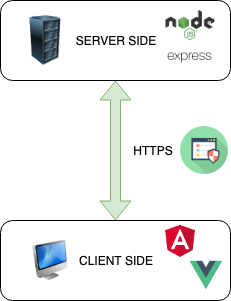
\includegraphics[scale=0.8]{images/nodejs/app_working.png}
	\caption{Ogólny schemat działania aplikacji typu klient-serwer bazującej na serwerze \textit{Node.js} oraz nowoczesnych frameworkach implementacji warstwy prezentacji}
	\label{Rys:nodejs}
\end{figure}

\section{Implementacja aplikacji serwerowej}
W poniższym rozdziale przedstawiony zostanie sposób implementacji aplikacji serwerowej bazującej na zestawie bibliotek \textit{Node.js} oraz \textit{Express.js}.

\subsection{Inicjalizacja serwera}
Inicjalizacja serwera rozpoczyna się od wygenerowania do celów testowych klucza i certyfikatu auto-podpisanego SSL (\textit{Secure Socket Layer}), który używany jest przez protokół HTTPS (\textit{Hypertext Transfer Protocol Secure}) w celu zwiększenia bezpieczeństwa danych. Kolejnym krokiem jest zdefiniowanie portu, na który będą kierowane żądania klienta i rozpoczęcia nasłuchiwania. W tym celu posłużono się frameworkiem \textit{Express.js} i zdefiniowano lokalny serwer HTTPS pracujący na porcie numer 9000. 

W celu wygenerowania certyfikatu i klucza RSA (\textit{Rivest-Shamir-Adleman}) posłużono się poniższą komendą:

\begin{figure}[h]
	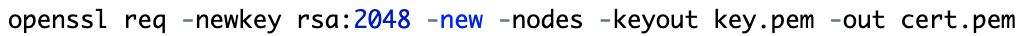
\includegraphics[scale=0.7]{images/code/openssl_newkey.png}
	\label{Rys:nodejs}
\end{figure}

Wygenerowany klucz RSA zawiera 2048 bitów. Klucze mniejsze niż 2048 bitów nie są obecnie uważane za bezpieczne. Wersje 2048 bitowe mają wystarczającą liczbę unikalnych kodów szyfrowania. 

Sama, wstępna implementacja serwera HTTPS nasłuchującego na porcie o numerze 9000 i przekazanie wygenerowanych plików \textit{key.pem} oraz \textit{cert.pem} do parametrów inicjalizacji serwera  zaprezentowana została na poniższych blokach kodu źródłowego:

\begin{figure}[h]
	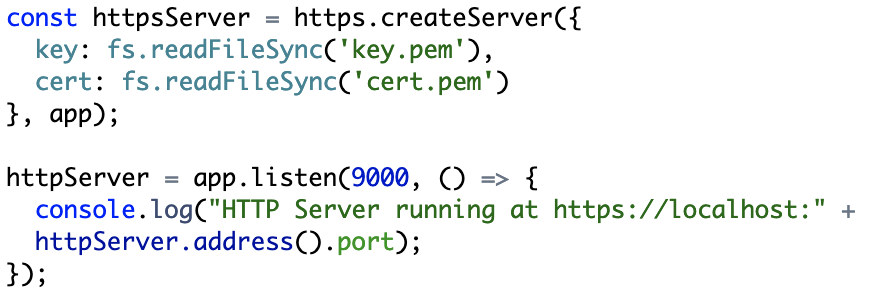
\includegraphics[scale=0.7]{images/code/create_server.png}
	\label{Rys:nodejs}
\end{figure}

W następnym kroku zdefiniowano komendę \textit{start-server}, za pomocą której uruchamiany będzie serwer. Definicja komendy znajduje się w pliku JSON służącym do zarządzania lokalnymi paczkami NPM (\textit{Node Package Module}) - \textit{package.json}. W celu uruchomienia serwera wystarczy użyć polecenia \textit{npm run start-server} w oknie terminala. 

\begin{figure}[h]
	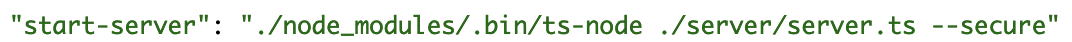
\includegraphics[scale=0.7]{images/code/start_server.png}
	\label{Rys:nodejs}
\end{figure}

Po uruchomieniu serwera z poziomu konsoli otrzymano komunikat widoczny na rysunku \ref{Rys:nodejs-running}. Oznacza on, że serwer został poprawnie uruchomiony i rozpoczęto nasłuchiwanie:

\begin{figure}[h]
	\centering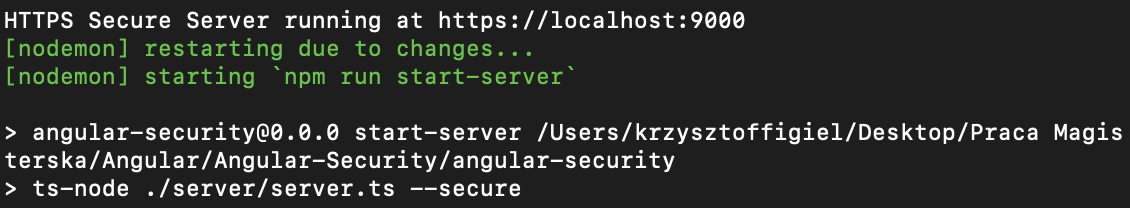
\includegraphics[scale=0.76]{images/nodejs/server-running.png}
	\caption{Zrzut ekranu konsoli systemu \textit{MacOS} ukazujący komunikaty o poprawnym uruchomieniu procesu nasłuchiwania przez serwer na porcie 9000}
	\label{Rys:nodejs-running}
\end{figure}

Definicja tabel routingu w \textit{Express.js} opiera się na użyciu funkcji \texttt{app.route(path)}. W aplikacji serwerowej zdefiniowano następujące ścieżki routingu:

\begin{itemize}
	\item \textit{/api/books}
	\item \textit{/api/signup}
	\item \textit{/api/user}
	\item \textit{/api/logout}
	\item \textit{/api/login}
\end{itemize}

Dane zawarte w tabelach routingu umożliwią 

Przykładowa definicja wpisu tabeli routingu zaprezentowana została na poniższym bloku kodu źródłowego:

\begin{figure}[h]
	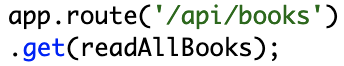
\includegraphics[scale=0.7]{images/code/app_route.png}
	\label{Rys:nodejs}
\end{figure}

Po poprawnym uruchomieniu aplikacji działającej na serwerze, włączonej na porcie lokalnym \textit{https://localhost:4200} otrzymano informację o tym, że przeglądarka używa zaszyfrowanego połączenia z \textit{localhost}:

\begin{figure}[h]
	\centering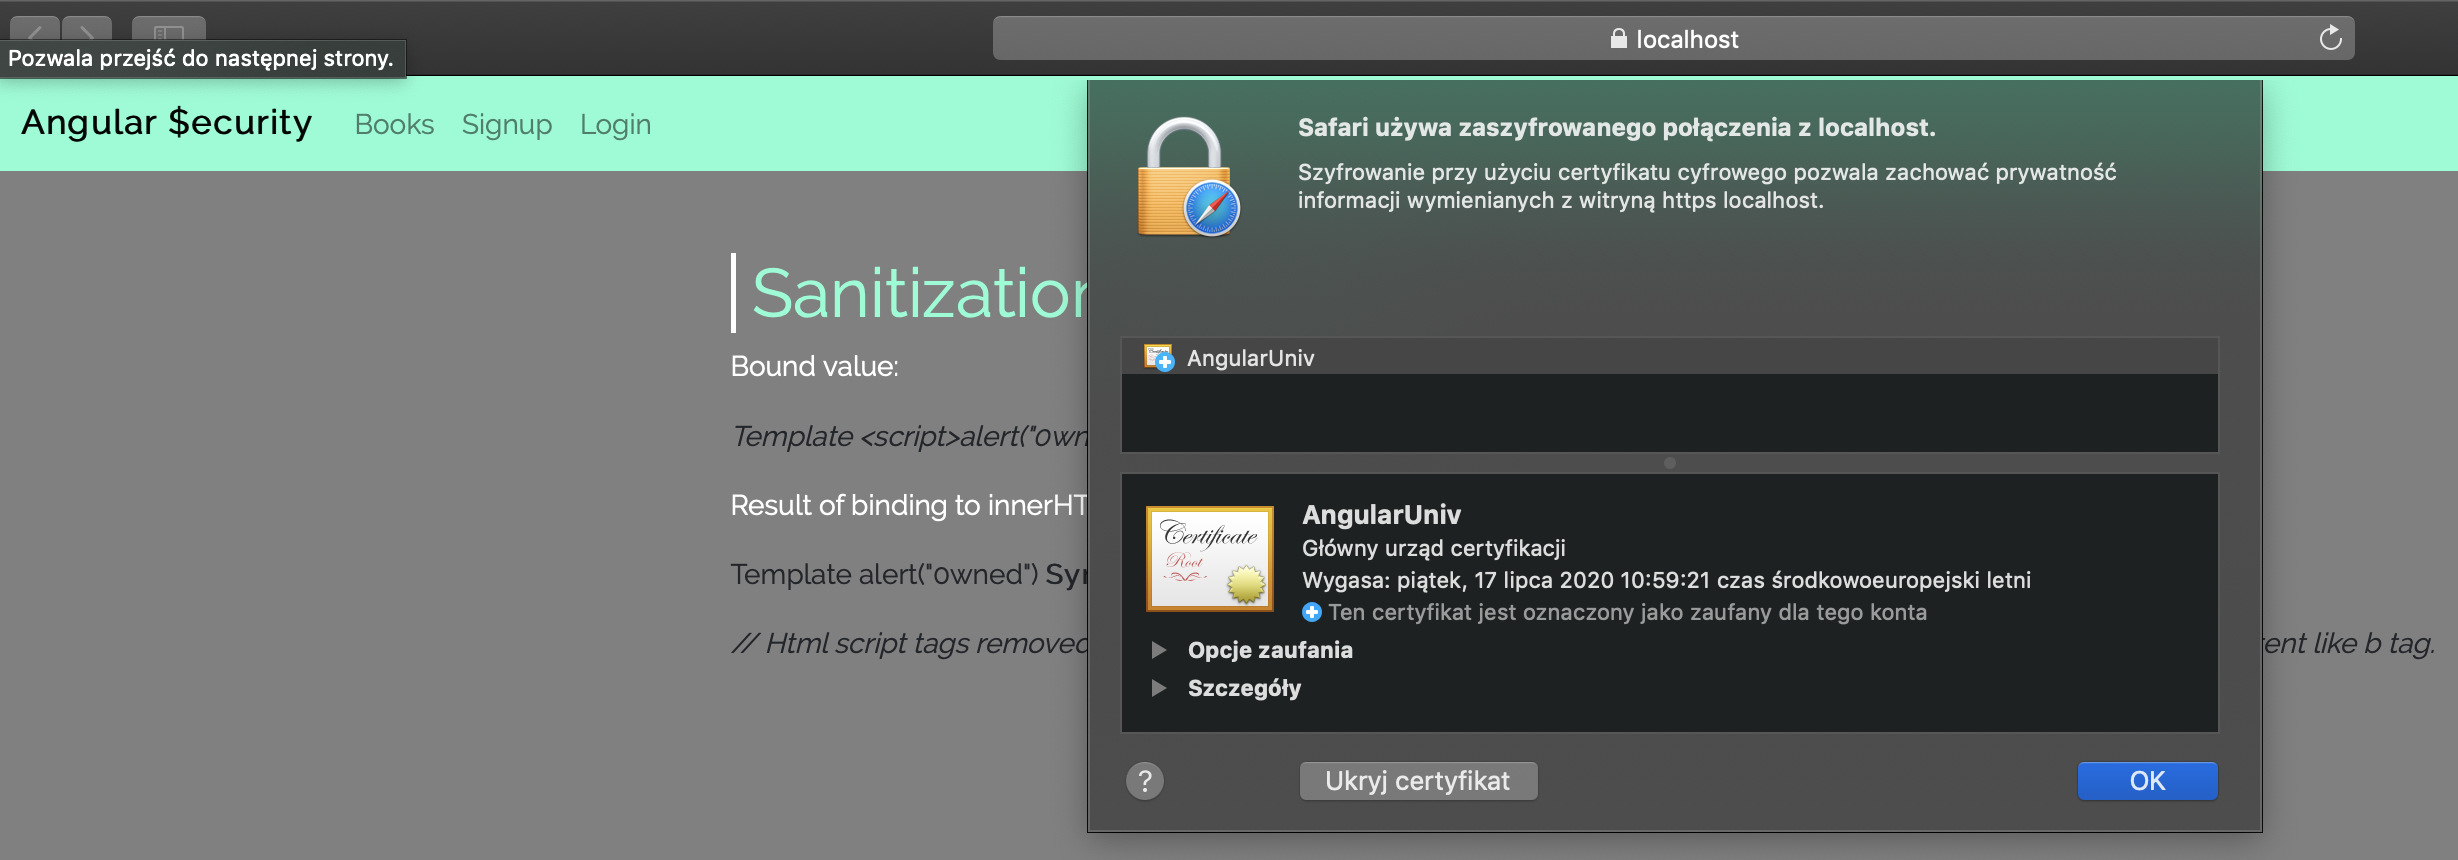
\includegraphics[scale=0.35]{images/nodejs/secure-cert.png}
	\caption{Okno przeglądarki internetowej \textit{Safari} ukazujące informację o poprawnym zaszyfrowaniu lokalnego połączenia aplikacji na porcie 4200 przy użyciu certyfikatu autopodpisanego.}
	\label{Rys:nodejs}
\end{figure}

\subsection{Implementacja modułu rejestracji nowego użytkownika} 
W następnym kroku zdefiniowano metody odpowiedzialne za obsługę rejestracji nowego użytkownika w aplikacji. Wpis tabeli routingu zawierający ścieżkę do tworzenia nowego użytkownika wygląda następująco:

\begin{figure}[h]
	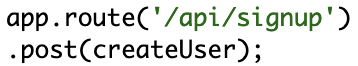
\includegraphics[scale=0.7]{images/code/app_route_user.png}
	\label{Rys:nodejs}
\end{figure}

Po zdefiniowaniu wpisu przystąpiono do implementacji metody \texttt{createUser(req, res)}. Sama implementacja tej metody opiera się na odebraniu parametrów przesyłanych przez użytkownika w obiekcie \texttt{req} i przekazania odpowiednich statusów metody HTTP do klienta (\texttt{res}) w zależności czy weryfikacja nowego użytkownika przebiegła pomyślnie czy też nie. 

Do walidacji haseł użytkownika posłużono się walidatorem z repozytorium NPM (\textit{Node Package Manager}) - \textit{password-validator}. Umożliwia on zdefiniowanie reguł tworzenia nowych haseł oraz dodawanie haseł, które znaleźć się mają na tzw. \textit{blacklist} czyli liście haseł niedopuszczalnych, powszechnie używanych. W celu zachowania bezpieczeństwa systemu zdefiniowano reguły i przykład \textit{blacklist} tworzenia nowych haseł przez użytkowników:

\begin{figure}[h]
	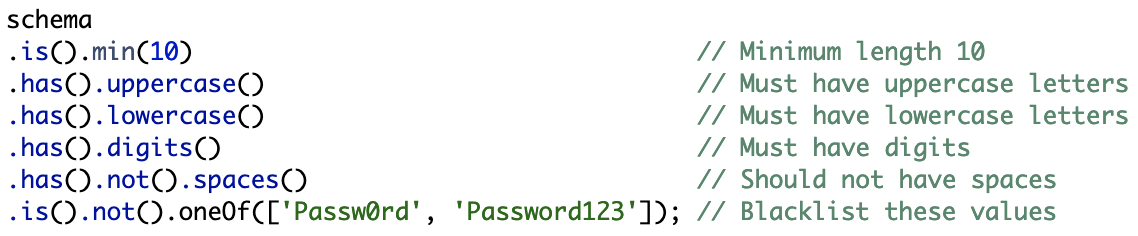
\includegraphics[scale=0.7]{images/code/passwords_schema.png}
\end{figure}

Po pomyślnej walidacji przesyłanego przez użytkownika w obiekcie \texttt{req} hasła serwer odpowiada komunikatem z kodem odpowiedzi HTTP o numerze 200 (\textit{OK}) przesyłając w parametrze \texttt{body} dane (\textit{id} oraz \textit{email}) nowego użytkownika. W tym celu posłużono się metodą \texttt{res.status(httpCode)}:

\begin{figure}[h]
	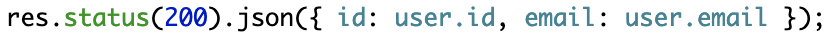
\includegraphics[scale=0.7]{images/code/res_status_200.png}
\end{figure}

W przypadku podania hasła niezgodnego z przyjętymi regułami tworzenia nowych haseł użytkownika serwer odpowiada komunikatem z kodem odpowiedzi HTTP o numerze 400 (\textit{Bad request}). Wykorzystano metodę \texttt{res.status(httpCode)}, a jako zwracany parametr podano listę błędów zwracaną przez pakiet \textit{password-validator}:

\begin{figure}[h]
	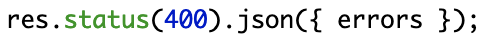
\includegraphics[scale=0.7]{images/code/res_status_400.png}
\end{figure}

Jeżeli serwer napotkał wewnętrzny błąd, wówczas wysyła on komunikat z kodem odpowiedzi HTTP o numerze 500 (\textit{Internal Server Error}) za pomocą metody \texttt{res.sendStatus(httpCode)} bez przekazywania treści błędu w celu zachowania odpowiedniej hermetyzacji aplikacji:

\begin{figure}[h]
	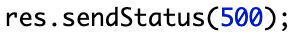
\includegraphics[scale=0.7]{images/code/res_status_500.png}
\end{figure}

Nowi użytkownicy przechowywani są w bazie danych za pomocą obiektu składającego się z trzech wartości:

\begin{figure}[H]
	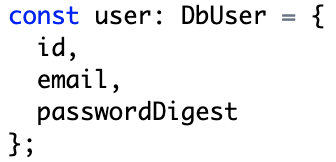
\includegraphics[scale=0.7]{images/code/db_content.png}
\end{figure}

Przy tworzeniu nowego użytkownika sprawdzany jest dodatkowo warunek czy nie ma już podobnego konta w bazie danych:

\begin{figure}[H]
	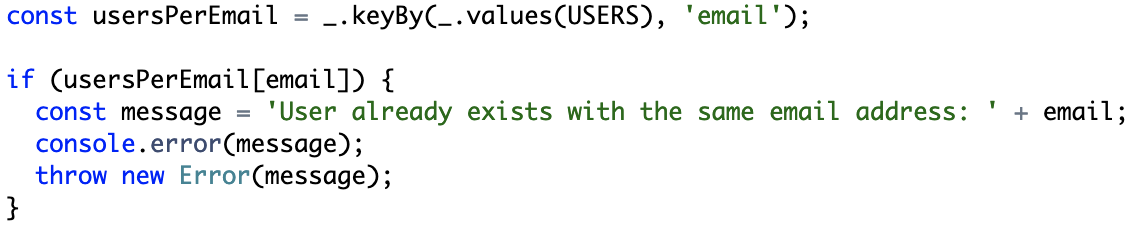
\includegraphics[scale=0.7]{images/code/user_exists.png}
\end{figure}

Jeżeli użytkownik istnieje w bazie danych wyświetlany jest stosowny komunikat. Serwer wysyła również do klienta odpowiedź z kodem statusu HTTP o numerze 500. Cały mechanizm zapobiega tworzeniu duplikatów użytkowników w bazie danych i uniemożliwia podszywanie się pod inne osoby widniejące w systemie. W przypadku braku podobnego konta i pomyślnej weryfikacji tworzony i zwracany jest nowy obiekt \texttt{user} a licznik użytkowników jest inkrementowany:

\begin{figure}[H]
	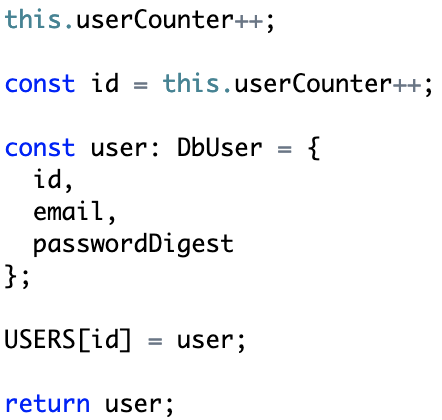
\includegraphics[scale=0.7]{images/code/new_user.png}
\end{figure}

Hasła użytkownika przechowywane są w bazie danych za pomocą funkcji skrótu \textit{Argon2}. W tym celu wykorzystano specjalny pakiet oferowany przez repozytorium NPM. Hasło podane przez użytkownika przekazywane jest jako parametr funkcji \texttt{argon2.hash(\textit{password})}. Więcej informacji na temat wykorzystania funkcji \textit{Argon2} zawarte zostało w rozdziale dotyczącym bezpieczeństwa. 

\subsection{Implementacja modułu logowania użytkownika}
Po zaimplementowaniu modułu rejestracji użytkownika stworzono moduł logowania. W tym celu, na samym początku dodano wpis do tabeli routingu z następującą ścieżką:

\begin{figure}[H]
	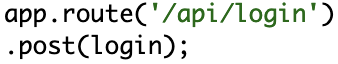
\includegraphics[scale=0.7]{images/code/app_route_login.png}
\end{figure}

W następnym kroku zaimplementowano funkcję \texttt{login(req: Request, res: Response)} odpowiedzialną za procedurę logowania. W środku funkcji następuje sprawdzanie, czy podane w parametrze dane użytkownika występują w bazie danych czy też nie (metoda \texttt{db.findUserByEmail}). W przypadku, gdy osoby nie ma w bazie zwracany jest kod HTTP o numerze 403 ze stosowną informacją zwrotną. 

Jeżeli użytkownik widnieje w systemie wywoływana jest metoda \texttt{loginAndBuildResponse}, zwracająca w przypadku poprawnego logowania odpowiedni kod odpowiedzi HTTP o numerze 200. Wówczas następuje dodanie tokena sesji o nazwie \textit{SESSIONID} do zawartości \textit{cookie} przeglądarki internetowej (Rys: \ref{Rys:cookie_sessionID}):

\begin{figure}[H]
	\centering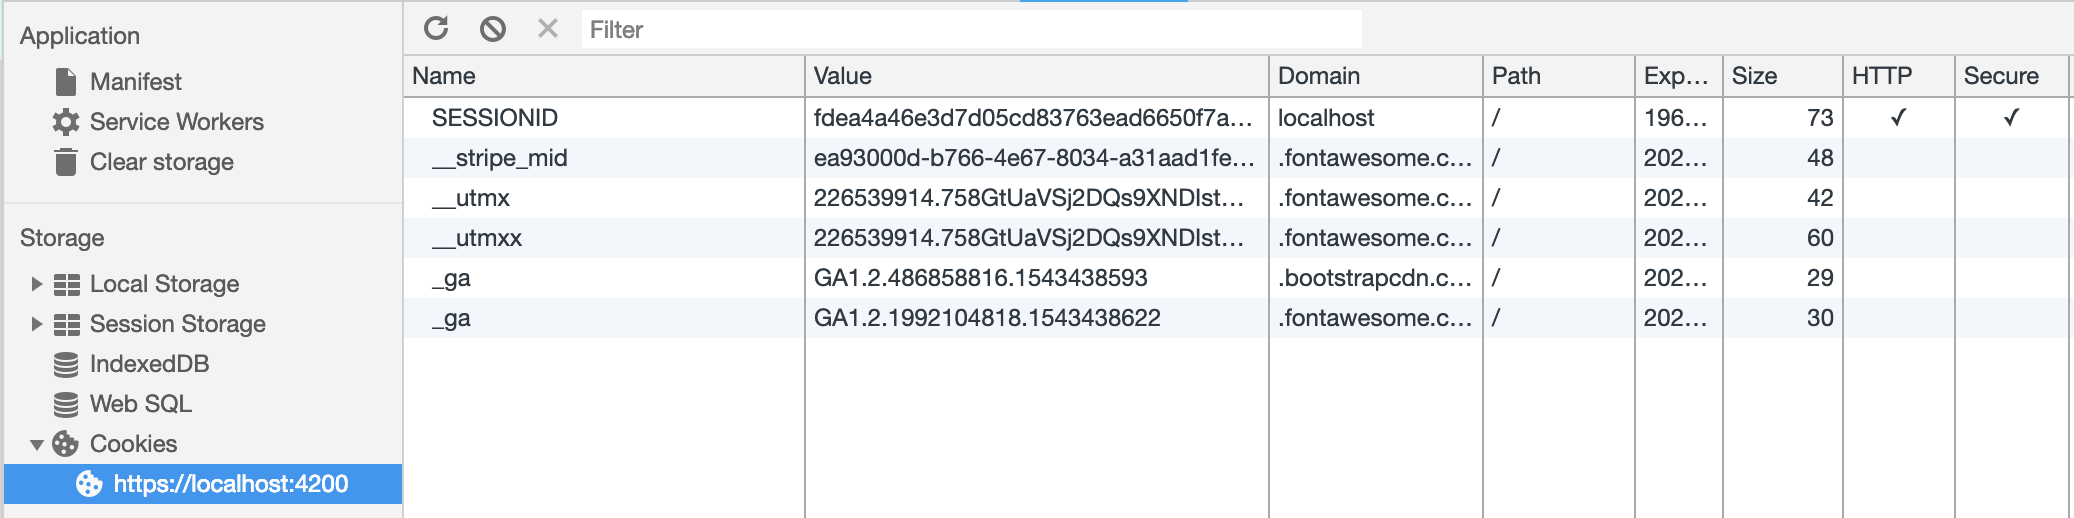
\includegraphics[scale=0.4]{images/nodejs/cookie_secure.png}
	\caption{Okno narzędzi deweloperskich (zakładka \textit{Application/Cookies}) przeglądarki internetowej \textit{Google Chrome} z dodanym tokenem sesyjnym \textit{SESSIONID} użytkownika}
	\label{Rys:cookie_sessionID}
\end{figure}

Sama implementacja tworzenia tokena sesji użytkownika i zapisywania go do ciasteczka przeglądarki wygląda następująco:

\begin{figure}[H]
	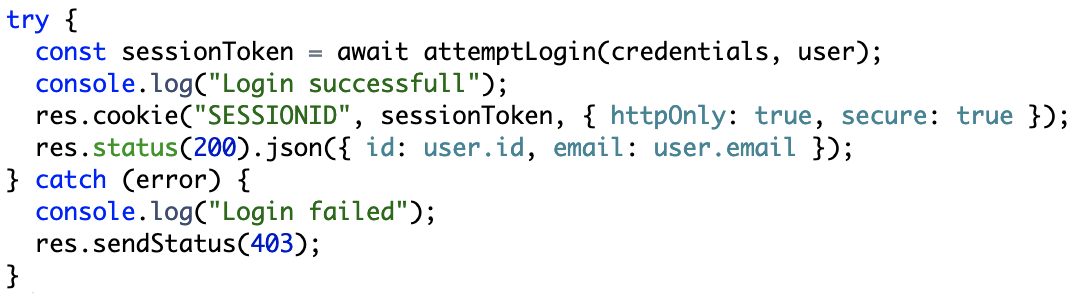
\includegraphics[scale=0.7]{images/code/add_cookie.png}
\end{figure}

Dzięki temu połączenie jest dodatkowo uwierzytelniane, a użytkownik ma wyłączność na korzystanie z własnej sesji danej witryny internetowej. Dodatkowo, token zapewnia podtrzymanie sesji użytkownika na pewien odstęp czasu (\textit{timestamp}). Więcej informacji na temat działania tokenu sesji zawarto w rozdziale czwartym dotyczącym mechanizmów bezpieczeństwa aplikacji internetowych opartych na języku \textit{JavaScript}.

\subsection{Implementacja modułu wylogowywania użytkownika}
Moduł wylogowywania również posiada własną ścieżkę w tabeli routingu. Jej implementacja wygląda następująco:

\begin{figure}[H]
	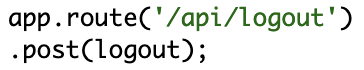
\includegraphics[scale=0.7]{images/code/res_logout.png}
\end{figure}

Jego działanie zaimplementowano w prosty sposób - całość opiera się na usunięciu tabeli ciasteczek sesyjnych (\textit{cookie}) w przeglądarce. Wiąże się to z usunięciem informacji o sesji użytkownika. Przy odpowiednim obsłużeniu wyniku działania tego modułu z poziomu warstwy aplikacji można w bardzo prosty sposób zablokować dostęp do treści strony, po ówczesnym wylogowaniu. Środowisko \textit{Node.js} umożliwia szybkie wyczyszczenie tabeli \textit{cookie} za pomocą metody \texttt{clearCookie()}:

\begin{figure}[H]
	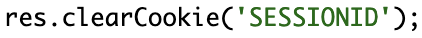
\includegraphics[scale=0.7]{images/code/clear_cookie.png}
\end{figure}

Czyszczenie zawartości tabeli ciastek sesyjnych przeglądarki jest konieczne z punktu widzenia bezpieczeństwa. Zapobiega to przechwyceniu informacji przez osoby trzecie, np. za pomocą ataku XSS (\textit{Cross-site scripting}). Mimo wszystko, nawet po uzyskaniu zawartości ciasteczka sesyjnego osoba atakująca napotka problem rozszyfrowania zawartych tam danych, które przechowywane są w postaci funkcjo skrótu \textit{Argon2}.

\begin{figure}[H]
	\centering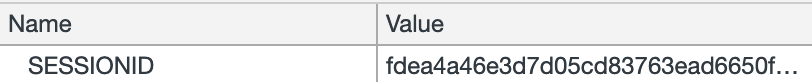
\includegraphics[scale=1.0]{images/nodejs/argon2_cookie.png}
	\caption{Okno narzędzi deweloperskich (zakładka \textit{Application/Cookies}) przeglądarki internetowej \textit{Google Chrome} z dodanym tokenem sesyjnym \textit{SESSIONID} użytkownika przechowywanym za pomocą funkcji skrótu \textit{Argon2}}
	\label{Rys:cookie_sessionID}
\end{figure}

\subsection{Implementacja mechanizmów podtrzymywania sesji użytkownika}
